\chapter{システム概要}
本研究では,VRを用いてユーザーの魔法体験における没入感を向上させるシステムを提案・開発し,視覚エフェクトと振動刺激の組み合わせによってユーザーの没入感にどのような影響を与えるのかを調査する.

\section{システム概要}
\figref{allsystem}に本システムの概要を示す.
\begin{figure}[h]
\centering
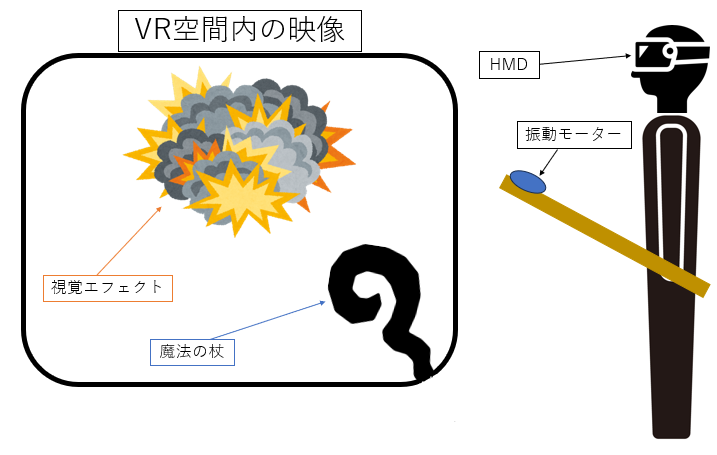
\includegraphics[clip,width=9cm]{./fig/allsystem.png}
\caption{システム概要}\label{allsystem}
\end{figure}

本研究では,被験者が右手にコントローラーを持った状態でHMDを装着する.
被験者がコントローラに装着されている押しボタンを押すことで視覚エフェクトと振動刺激が被験者に提示される.
提示する視覚エフェクトと振動刺激は実験者がPCから決定する.

\section{振動提示手法}
本研究では,振動提示の方法として振動モーターを使用した.
振動モーターをガムテープで木の角材に固定する.
被験者がこの角材を把持することによって角材を媒体とし被験者の手に伝わることで振動を提示できるようにした.

\section{魔法エフェクトの選定}
実装する視覚エフェクトは,形状が異なりユーザーに与えられる振動刺激が異なると思われる3種類の視覚エフェクトを選定した.

以下に選定した3種類の視覚エフェクトを示す.

incenerationを\figref{fire}に示す.incenerationは火が燃え続けるエフェクトである.
main-beamを\figref{explosion}に示す.main-beamは最初に大きな爆発があり,その後爆発の余韻が残るエフェクトである.
ring-fireを\figref{ringfire}に示す.ring-fireは初めにエネルギーをためるフェーズがあり,その後ためたエネルギーを一気に解放するエフェクトである.

\begin{figure}[h]
\centering
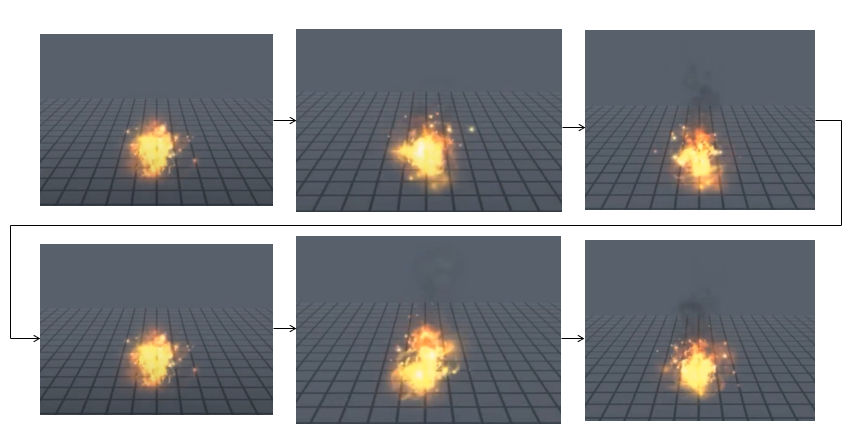
\includegraphics[clip,width=10cm]{./fig/fireTime.png}
\caption{inceneration}\label{fire}
\end{figure}

\begin{figure}[h]
\centering
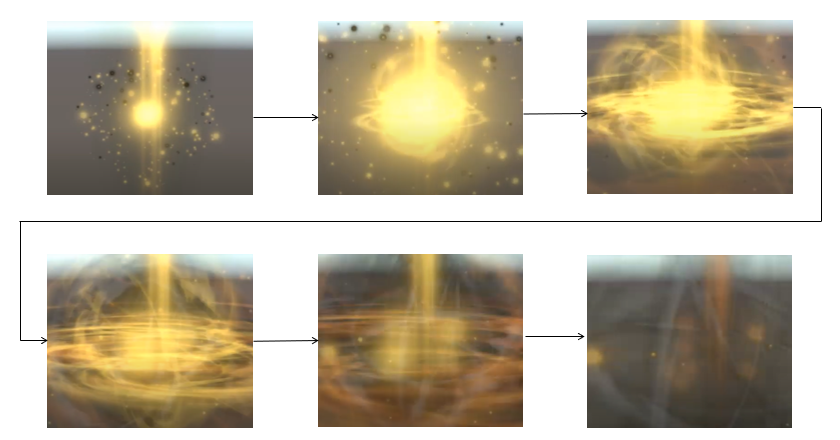
\includegraphics[clip,width=10cm]{./fig/mainbeamTime.png}
\caption{main-beam}\label{explosion}
\end{figure}

\begin{figure}[h]
\centering
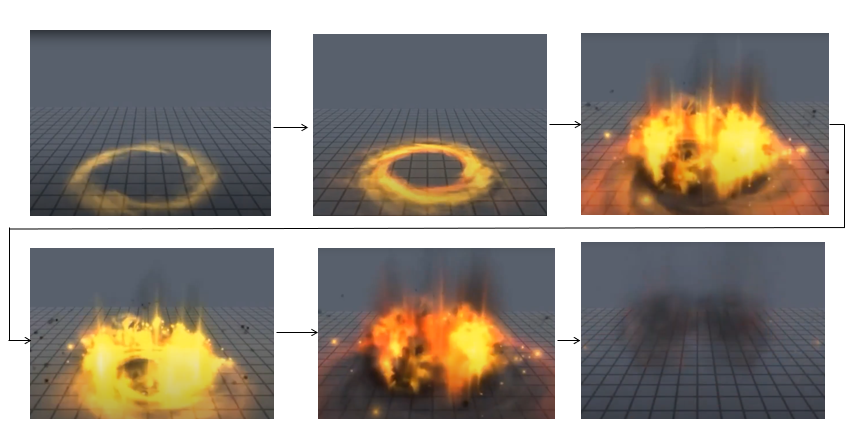
\includegraphics[clip,width=10cm]{./fig/ringfireTime.png}
\caption{ring-fire}\label{ringfire}
\end{figure}


\newpage
\subsection{振動パターンの選定}
以下に選定した4種類の振動パターンを示す.
振動強度が一定,弱~強,強~弱,矩形波の4種類である.
それぞれ順にパターン1パターン2パターン3パターン4とする.
対応表を\ref{tab;sindou}に示す.

矩形波とは,波形を時間領域で見たときに方形状を持つ波のことである.
振動が一定間隔で高低2つの一定値を繰り返す.
本研究では低い振動を振動させないようにしている.
そのため一定期間で振動モーターが動いたり止まったりを繰り返す挙動をとる.

\begin{table}[H]
    \caption{振動パターン対応表}
    \centering
    \begin{tabular}{l|l}
    \hline
    \hline
    パターン1 & 一定 \\
    パターン2 & 弱→強 \\
    パターン3 & 強→弱 \\
    パターン4 & 矩形波 \\
    \hline
    \end{tabular}
    \label{tab;sindou}
\end{table}


\begin{figure}[h]
\centering
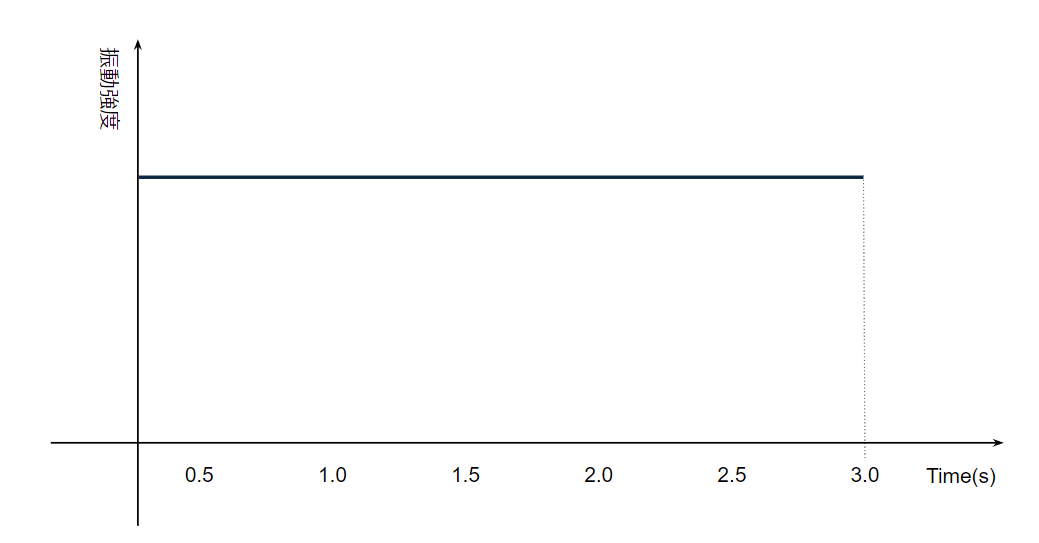
\includegraphics[clip,width=10cm]{./fig/patarn1.png}
\caption{パターン1}\label{patarn1}
\end{figure}

\begin{figure}[h]
\centering
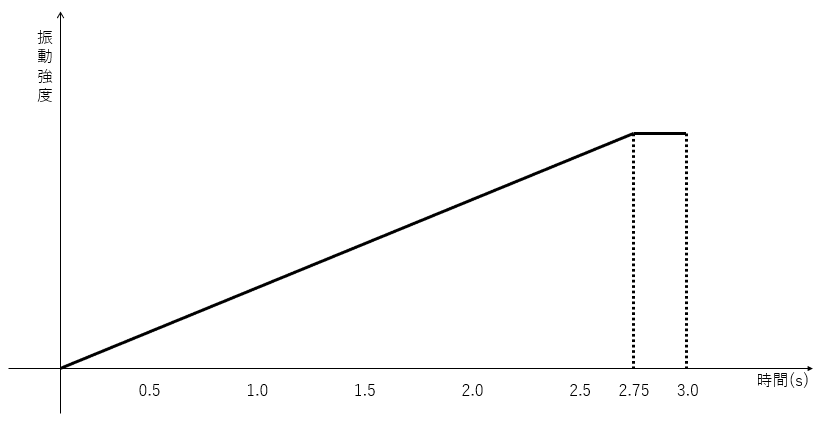
\includegraphics[clip,width=10cm]{./fig/patarn2.png}
\caption{パターン2}\label{patarn2}
\end{figure}

\begin{figure}[h]
\centering
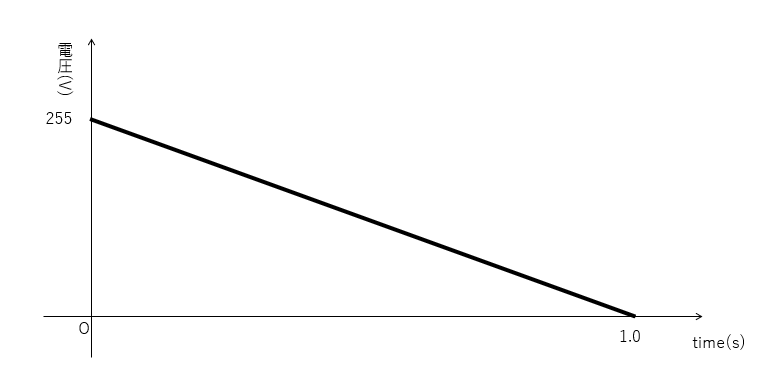
\includegraphics[clip,width=10cm]{./fig/patarn3.png}
\caption{パターン3}\label{patarn3}
\end{figure}

\begin{figure}[h]
\centering
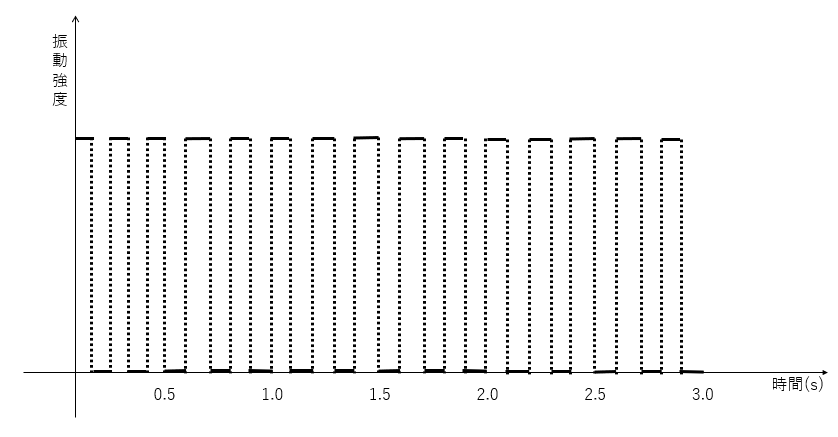
\includegraphics[clip,width=10cm]{./fig/patarn4.png}
\caption{パターン4}\label{patarn4}
\end{figure}


